\dev{Emile Martinez}{}

\section{Introduction}

\subsection{Définition}

\begin{definition}
	On dit que un algorithme apprend via un entraînement pour un ensemble de tâches et une mesure de performance si sa performance sur les tâches mesuré par la mesure de performance s’améliore après l'entraînement.
\end{definition}

\begin{definition}
	\label{15-def-1}
	On considère deux familles de l’apprentissage machine :
	\begin{enumerate}
		\item l’apprentissage supervisé : on dispose d’espaces $X$ d’entrée et $Y$ de sortie, et d’un ensemble $E$ d’exemples $(x_i , y_i ) \in X \times Y$, représentant une fonction $f : X \to Y$. Le but étant alors de construire une fonction $\hat{h} : X \to Y$ approximant $f$.
		\item l’apprentissage non supervisé : on dispose seulement de l’espace $X$  dont on veut alors découvrir les structures sous-jacente
	\end{enumerate}
\end{definition}

\begin{example}
	Sur un ensemble de données sur des animaux, on peut :\begin{enumerate}
		\item Savoir lesquels sont des chiens, des chats, etc... (apprentissage supervisé)
		\item Savoir quels animaux sont de la même espèce (apprentissage non supervisé)
	\end{enumerate}
\end{example}

\begin{rem}
	Il existe d’autres familles, comme l’apprentissage par renforcement qui consiste à maximiser un critère d’utilité par expériences successives.
\end{rem}

\subsection{Évaluation d'un algorithme d'apprentissage}
\label{15-I-2}

On cherche à évaluer la performance d'un algorithme d'apprentissage.

\begin{definition}
	On découpe nos données d'entrées $E$ en deux :
	\begin{itemize}
		\item Les données d'apprentissage, servant à entraîner l'algorithme
		\item Les données de validation, servant à imiter la prédiction, mais en comparant le résultat obtenu à celui attendu.
	\end{itemize}
\end{definition}

\begin{rem}
	Si l'on a trop peu de données, on peut également faire une validation croisée, consistant utiliser alternativement des données comme apprentissage et comme validation
\end{rem}

\begin{rem}
	Cette phase est également utile pour calibrer les paramêtres de l'algorithme.
\end{rem}

\section{Apprentissage supervisé}

On reprend les notations de la définition \ref{15-def-1}

\begin{com}
	Dans un vrai cours, on réécrirait les définitions pour plus de clarté
\end{com}

\begin{definition}\enspace
	
	Si $Y$ est un ensemble fini de classes, on parle de problème de classification.
	
	Si $Y =\mathbb R$, on parle de problèmes de régression.
\end{definition}

\begin{example}
	Sur un ensemble de données sur des animaux, on peut avoir : \begin{itemize}
		\item $Y = \{'chien', 'chat'\}$ (classification)
		\item $Y = \mathbb R$ représentant le poids de l'animal (régression)
	\end{itemize}
\end{example}

Concentrons nous sur le problème de classification. On cherche à inférer de $E$, la classe de $\alpha \in X$. Notons $C$ la partition de $X$ représentant les différentes classes.

\subsection{$K$ plus proches voisins}

On s'intéresse ici au cas où $X = \mathbb R^d$

\begin{algo}
	K plus proches voisins de $\alpha$
	\begin{enumerate}
		\item Déterminer les $K$ plus proches voisins de $\alpha$ dans $E$
		\item Choisir la classe majoritaire parmi ces voisins.
	\end{enumerate}
\end{algo}

\textbf{Développement :} Présentation de l'algorithme illustrant différents aspects de l'apprentissage machine.

\begin{example}\enspace\\
	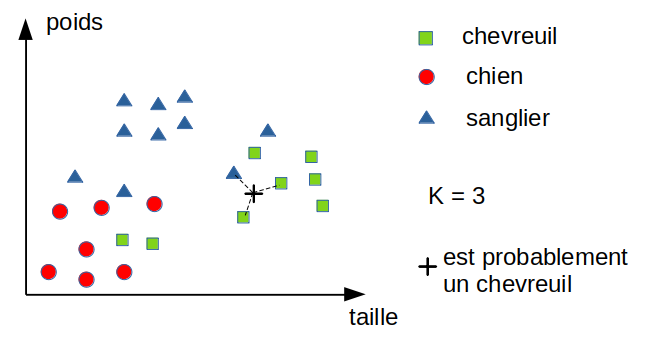
\includegraphics[width=0.6\linewidth]{lecon/15-ml/graphe.png}
\end{example}

\begin{rem}
	Ici pour choisir k, on utilise la méthode de mesure de performance du \ref{15-I-2} en essayant plusieurs paramètres.
\end{rem}

\begin{exercise}
	Appliquer l'algorithme sur le jeu de données MINST.
\end{exercise}

\begin{rem}
	Pour un problème de régression, on ne choisirait pas la classe majoritaire à l'étape 2, mais on agrégerait les données (par exemple en faisant une moyenne).
\end{rem}

\begin{impl}\enspace
	
	\textbf{Solution initiale :} Stocker nos $K$ valeurs en cours dans une file de priorité (implémentée par un tas max) et parcourir les $n$ points en mettant à jour la file de priorité
	
	\textbf{Complexité :} $O(n\log k)$\\
	
	\textbf{Solution diviser pour régner :} Faire un pré traitement où l'on stockera nos valeurs dans un arbre binaire de recherche (arbre $d$-dimensionnel), où l'on partitionnera récursivement les données alternativement sur chaque dimension. La recherche se fait alors en ne cherchant que d'un côté si le deuxième n'est pas nécessaire.
	
	\textbf{Complexité :}\\
	Prétraitement :$O(n \log n)$\\
	Recherche des k voisins : $O(k \log n)$ en moyenne et $O(nk)$ dans le pire des cas.
\end{impl}

\noindent \textbf{Développement :} Présentation de la structure d'arbre $d$-dimensionnel.

\begin{rem}
	On parle souvent d'arbre $k$-dimensionnel, mais on prend ici $d$ pour éviter la confusion avec $K$.
\end{rem}

\subsection{Arbre de décision}

On s'intéresse ici au cas $X = \mathbb R^d$ (ou $\{O, 1\}^d$)

\begin{idee}
	Partitionner récursivement X grâce à un arbre de décision où chaque feuille a une classe.\\
	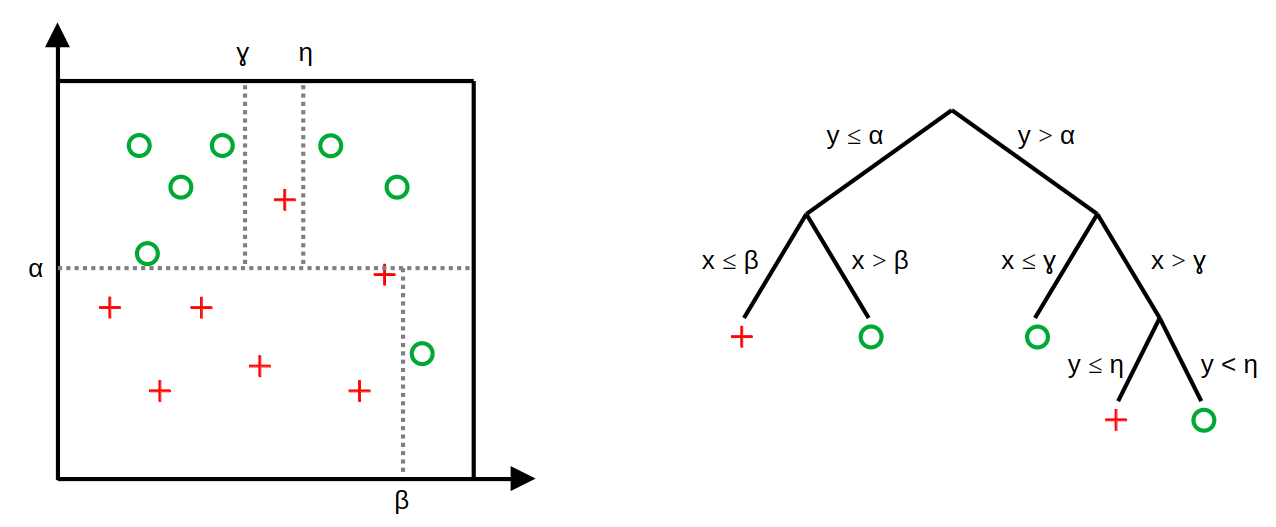
\includegraphics[width=\linewidth]{lecon/15-ml/arb_dec.png}
\end{idee}

\begin{definition}
	Définissons l'entropie d'une partie $S$ de $E$ : $H(S) = \sum\limits_{c \in C} \dfrac{|S\cap c|}{|S|} \times \log\left(\dfrac{|S\cap c|}{|S|}\right)$
\end{definition}

\begin{rem}
	Si tous les éléments ont la même classe, $H(S) = 0$
\end{rem}

\begin{definition}
	Le gain d'une partition $S_1$, $S_2$ de $S$ est : $$H(S) - \left( \dfrac{|S_1|}{|S|} \times H(S_1) + \dfrac{|S_2|}{|S|} \times H(S_2) \right)$$	
\end{definition}

\begin{algo}
	On construit récursivement notre arbre de décision sur notre ensemble S de données restantes:
	\begin{itemize}[label=$\bullet$]
		\item Si $S$ est vide : Choisir la classe la plus représentée du nœud parent
		\item Si toutes les données de $S$ ont la même classe : en faire une feuille avec cette classe.
		\item Sinon, on choisit la coordonnée $i$ et la valeur $m$ tel que la partition $$ S_1 = \left\{ (x_1, \dots, x_n) \in S / x_i \leq m\right\} \text{ et } S_2 = \left\{ (x_1, \dots, x_n) \in S / x_i > m\right\}$$ maximise le gain
	\end{itemize}
\end{algo}

\begin{rem}
	On atteint très vite du sur apprentissage. Pour éviter cela, on peut élaguer le bas de l'arbre (algorithme de Cart)
\end{rem}

\begin{exercise}
	Application à détecter la langue d'une page wikipedia à partir de la matrice de fréquence de facteurs de 2 lettres.
\end{exercise}

\begin{com}
	Ici pour ce TD, on peut mentionner à l'oral le fait qu'on peut utiliser ce truc pour de vrais, et surtout que on peut éventuellement faire réfléchir les élèves à comment modéliser le problème. Fréquence des mots, KNN avec distance de levenstein, fréquence des facteurs de 1, 2, 5 lettres ? Ce qui rend tout ca très intéressants selon moi. (suivant le nombre de pages en exemples, on peut prendre les facteurs d'un certain nombres de lettres (on aura un tableau de taille $27^{\text{taille des facteurs}}$) et ensuite faire du KNN, de l'arbre de décision, etc...) (Avec 4000 pages par langues pour 13 langues, et les facteurs de 2 mots, on classifie très bien).
\end{com}

\begin{rem}
	Dans le cas d'une régression, on peut prendre comme mesure d'impureté la variance.
\end{rem}

\subsection{Représentation de la qualité des classes}

Quand on mesure la performance de notre algorithme on peut chercher à représenter la qualité de nos prédictions (pour classification).

\begin{definition}[matrice de confusion]
	On associe $Y$ à $\{1, \dots, n\}$. La matrice de confusion est alors la matrice carrée $M$ de taille $n$ tel que $M_{i,j}$ est le nombre d'éléments de la classe $i$ qui ont été classés à $j$
\end{definition}

\begin{proposition}
	Plus notre algorithme est correcte, plus la diagonale est dominante.
\end{proposition}

\section{Apprentissage non supervisé}

\begin{rem}
	Il existe plusieurs types d'apprentissage non supervisé. On peut par exemple penser à la réduction de dimension : On a $X\subset \mathbb R^n$ et on cherche $f : X \to \mathbb R^m$ avec $n < m$ et tel que $f(x)$ et $f(y)$ sont proches si $x$ et $y$ le sont aussi.
	
	On se concentrera sur ce qu'on appellera regroupement, (clustering en anglais, ou classification non supervisée) qui consiste à trouver $f : X \to \{1, ..., k\}$ essayant de regrouper les éléments les plus proches.
\end{rem}

\begin{example}
	On a un manuscrit dans un alphabet inconnu, et on cherche à savoir quels lettres sont les mêmes.
\end{example}

\begin{exercise}
	Dans l'exemple au dessus, quel $X$ prendre ?
\end{exercise}

\subsection{Classification hiérarchique ascendante}

\begin{idee}
	Chacun est seul dans sa classe au début, et tant qu'on a $k$ classes, on fusionne les classes les plus proches.
\end{idee}

\begin{rem}
	C'est un algorithme glouton
\end{rem}

\begin{rem}
	Pour définir la distance entre deux classes, on prendre prendre : \begin{itemize}[label=$\bullet$]
		\item $d(S_1, S_2) = \min\limits_{x \in S_1, y \in S_2} (d(x, y))$
		\item $d(S_1, S_2) = \min\limits_{x \in S_1, y \in S_2} (d(x, y))$
		\item $d(S_1, S_2)  = \dfrac{1}{|S_1| \times |S_2|} \sum\limits_{x \in S_1, y \in S_2} d(x, y)$
	\end{itemize}
\end{rem}

\begin{exercise}
	Activité : Représenter l'exécution de l'algorithme sur un dendrogramme
\end{exercise}

\subsection{ALgorithme des $k$-moyennes}

\begin{idee}
	On cherche à trouver $S_1, \dots, S_k$ une partition de $X$ et $z_1, \dots, z_k \in \mathbb R^d$ minimisant $\sum\limits_{i = 1}^{k} \sum\limits_{x \in S_i} d(x, z_i)$
\end{idee}

\begin{algorithm}
	\caption{K-mean}
	Assigner à chaque valeur une classe aléatoire\\
	\Repeter{stabilisation}
	{
		\Pour{$x \in X$}
		{
			assigner à $x$ la classe de $\argmin\limits_{i \in \{1, \dots, k\}} d(x, z_i)$
		}
		\Pour{$i$ allant de $1$ à $k$}
		{
			$z_i \gets \dfrac{1}{|S_i|} \sum\limits_{x \in S_i} x$
		}
	}	
\end{algorithm}

\begin{proposition}
	Cet algorithme termine
\end{proposition}

\begin{proof}
	La cible diminue à chaque étape, et ne peut prendre qu'un nombre fini de valeurs.
\end{proof}

\begin{rem}
	On ne trouve pas toujours le minimum, on tombe souvent dans un minimum local. On relance alors plusieurs fois l'algorithme (d'où l'aléatoire au début).
\end{rem}

\begin{exercise}
	TP sur la réduction de palette d'une image
\end{exercise}

\begin{rem}
	Comment choisir $k$ ? Pour la classification hierarchique ascendante, on s'arrête au plus grand saut sur le dendrogramme, pour les k-moyennes, on affiche la cible finale en fonction de $k$ , et on choisit $k$ au changement de pente.\\
	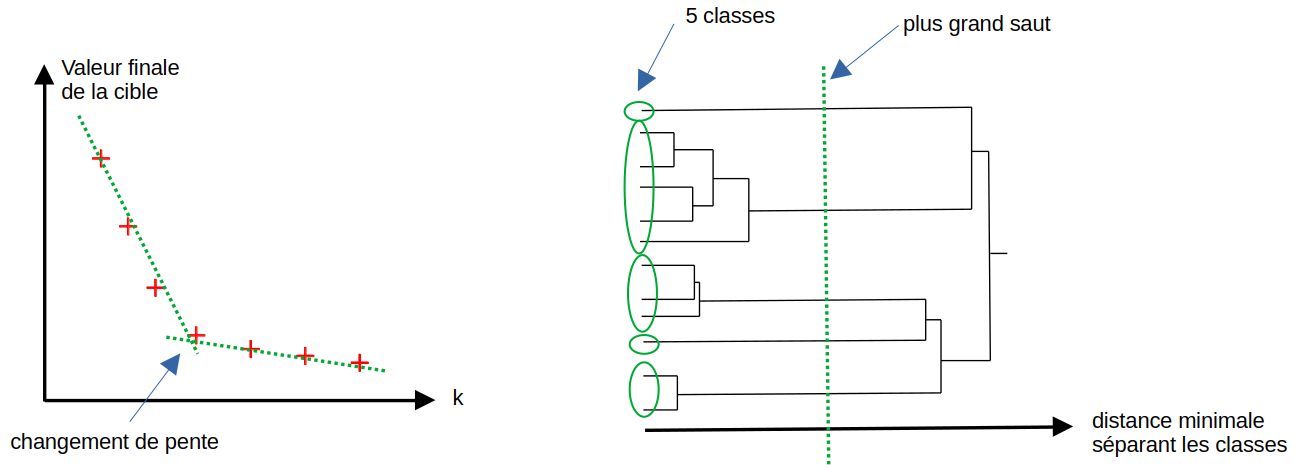
\includegraphics[width=\linewidth]{lecon/15-ml/choix_k.png}
\end{rem}

\begin{com}
	Si on a la place, on peut faire de cette remarque une sous-partie supplémentaire. Si on l'a pas, on peut enlever les dessins, et simplement le mentionner pour les k-moyennes, ou même l'enlever au pire.
\end{com}